\documentclass[11pt]{article}
\usepackage[margin=1in]{geometry}
\usepackage{booktabs,graphicx,amsmath,hyperref,microtype,authblk}
\usepackage[numbers,sort&compress]{natbib}
\hypersetup{colorlinks=true,linkcolor=blue,citecolor=blue,urlcolor=blue}

\title{Annotator Disagreement, Not Spatial Context, Bounds Pulmonary
Nodule Malignancy-Risk Classification on LIDC-IDRI}

\author[1]{Bahodir Nazarov}
\author[1]{Zaineb Gharib}
\author[1]{Fatima Zazoul}
\author[1]{Haixian Zhang}
\affil[1]{\small Sichuan University}
\date{}

\begin{document}
\maketitle

\begin{abstract}
Deep learning studies on LIDC-IDRI routinely report that richer spatial
context---moving from a single slice to a stack of slices to a full
volume---improves pulmonary nodule malignancy-risk classification. We test this
directly under a single controlled pipeline in which representation is the only
variable, and find no such benefit. Across 2D (one slice), 2.5D (five slices)
and 3D (full volume) encoders sharing identical preprocessing, patient-level
splits, loss, optimiser, augmentation, model-selection rule and metrics, all
representations converge to a three-class macro-F1 of approximately $0.60$.
Self-supervised MoCo~v2 pretraining on 5133 unlabelled training-patient nodules
produced no measurable gain in the 2D and 2.5D arms, and an apparent gain only
in the 3D arm, where validation did not reliably rank configurations. We show
instead that performance is bounded by \emph{annotator disagreement}. On a binary
benign-versus-malignant cohort drawn from the same images and patient splits,
accuracy is $0.945$ and AUC $0.987$ on nodules with concordant radiologist
labels, but falls to $0.805$ and $0.902$ on the remainder; classification
accuracy tracks the median malignancy rating, collapsing from $\sim\!0.90$ at
the rating extremes to $0.667$ at a median of $3.5$, a value that is not an
original radiologist rating but an artefact of averaging disagreeing readers.
Models are appropriately uncertain rather than confidently wrong, with mean
confidence $0.762$ on correct predictions against $0.462$ on errors. We argue
that a substantial part of the headroom commonly attributed to architecture on
this dataset is instead label noise, and that LIDC-IDRI results should be
reported stratified by annotator agreement.
\end{abstract}

\section{Introduction}

Computed tomography is volumetric, and a long line of work argues that deep
models should exploit that structure: 2.5D models stack neighbouring slices,
and 3D models consume whole volumes. Reported gains are usually modest and are
almost always confounded, because the compared systems differ not only in
spatial context but in preprocessing, intensity windowing, augmentation,
capacity, training schedule and evaluation protocol.

We ask a narrower question. \emph{If everything except the input representation
is held fixed, how much does spatial context actually contribute?} We build one
pipeline in which 2D, 2.5D and 3D arms share the same nodule crops, the same
Hounsfield-unit window, the same patient-level splits, the same class-weighted
loss, the same optimiser and schedule, the same augmentation recipe, the same
early-stopping criterion and the same metric code. The encoders differ only in
input dimensionality; the 2D and 2.5D models are the same ResNet-18 differing in
a single argument, \texttt{in\_channels}.

Our contributions:

\begin{enumerate}
\item Under this controlled comparison, added spatial context yields no
  improvement. Three-class macro-F1 is $0.6059 \pm 0.024$ (2D),
  $0.5785 \pm 0.022$ (2.5D) and $0.5653 \pm 0.041$ (3D), all within one to two seed
  standard deviations of one another.
\item MoCo~v2 pretraining on 5133 unlabelled training-patient nodules gives no
  measurable benefit in the 2D or 2.5D arms despite the pretext task itself
  converging well. It does improve the 3D arm by $+0.043$ macro-F1, but 3D
  validation ranked configurations inconsistently with test, so we treat this
  as an observation requiring more seeds rather than a result.
\item We locate the performance ceiling in annotator disagreement rather than
  model capacity, and quantify it: binary accuracy is $0.945$ / AUC $0.987$ on
  concordantly labelled nodules versus $0.805$ / $0.902$ on the remainder.
\item We show that augmentation does not reduce memorisation, and report the
  seed-variance reduction it does deliver.
\end{enumerate}

\section{Data}

We use LIDC-IDRI~\citep{armato2011lidc}, obtained through
TCIA~\citep{clark2013tcia}. Consensus nodules were extracted as
$104\times72\times80$ crops resampled to $1\,\mathrm{mm}$ isotropic spacing,
with the nodule at the geometric centre of every crop; the measured mask
centre-of-mass across random samples is $z \in [51.1, 52.1]$,
$y \in [35.2, 35.7]$, $x \in [39.3, 39.9]$.

\paragraph{Labels.} Each nodule carries malignancy ratings from up to four
radiologists on a 1--5 scale. We use the project three-class rule: median
$1.0$--$2.0$ is \emph{benign}, $2.5$--$3.0$ \emph{indeterminate}, and
$3.5$--$5.0$ \emph{malignant}. Crucially, medians of $2.5$ and $3.5$ are
\emph{not} radiologist ratings; they arise only when readers disagree. 449
nodules carry such midpoint medians, and we return to them in
Section~\ref{sec:ceiling}.

\paragraph{Cohorts.} The labelled cohort is 2654 nodules (873 benign, 1226
indeterminate, 555 malignant), split at patient level into 1876 / 382 / 396
nodules over 602 / 134 / 134 patients. A binary cohort excluding
\emph{indeterminate} gives 1000 / 219 / 209 nodules; it is a strict subset of
the same splits, so no patient moves between partitions. The self-supervised
pool is 5133 nodules from 692 training-split patients, used without labels; it
may include labelled training nodules but contains no validation or test
patient.

\paragraph{Leakage control.} We verified programmatically, and re-assert on
every training run, that no patient and no nodule appears in more than one
split, and that the self-supervised pool contains no validation or test patient.
The check raises rather than warns.

\section{Method}

\paragraph{Preprocessing (shared).} Stored volumes are raw Hounsfield units
with observed values from $-3024$ to $+3080$. We clip to $[-1000, 400]$, scale
to $[0,1]$, then standardise with training-split statistics. This window is
applied identically in all arms; it is the single most important shared choice,
since an unstated difference here would masquerade as a representation effect.

\paragraph{Representations.}
\begin{itemize}
\item \textbf{2D}: the central slice, $(1, 72, 80)$,
  ResNet-18~\citep{he2016resnet}.
\item \textbf{2.5D}: five neighbouring slices as channels, $(5, 72, 80)$,
  the same ResNet-18 with \texttt{in\_channels}$=5$.
\item \textbf{3D}: the full crop, $(1, 104, 72, 80)$, a 3D
  ResNet-10~\citep{hara2018spatiotemporal}.
\end{itemize}
The 2D and 2.5D models differ by 12{,}544 parameters, entirely in the first
convolution. We use ResNet-10 rather than ResNet-18 in 3D because a 3D
ResNet-18 would carry roughly 33M parameters against 1876 training volumes.

\paragraph{Training (shared).} AdamW~\citep{loshchilov2019adamw}, learning rate
$10^{-3}$, weight decay $0.05$, cosine schedule, batch 64 (16 in 3D), dropout
$0.5$, label smoothing $0.10$, inverse-frequency class weights, early stopping
with patience 20 on validation macro-F1, maximum 80 epochs. Learning rate,
weight decay, dropout and label smoothing were selected on validation only, by
a single-seed sweep of eight configurations in the 2D arm, and then frozen for
every other arm. Augmentation strength is not tuned; it is an experimental
factor (Models A--C below). The test split was never used for tuning or
checkpoint selection.

\paragraph{Models.} \textbf{A}: supervised from random initialisation, no
augmentation. \textbf{B}: MoCo~v2 pretraining, then supervised fine-tuning
without augmentation. \textbf{C}: as A, with the mild augmentation below. The
binary runs use the Model C recipe.

\paragraph{Augmentation.} Training only, Model C and binary runs. Horizontal
and vertical flips ($p=0.5$ each), a combined affine transform ($p=0.8$;
rotation $\pm15^\circ$, translation $\pm6\%$, scale $0.9$--$1.1$), intensity
jitter ($p=0.5$; multiplicative $0.9$--$1.1$ then additive $\pm0.05$) and
Gaussian noise ($p=0.3$, $\sigma=0.02$). A \emph{strong} variant, reported
only as an ablation, doubles the geometric ranges, triples the intensity
ranges, uses $\sigma=0.05$ and adds random erasing ($p=0.25$). In 3D, flips are
in-plane only, so the volume is never flipped along $z$. In the reported 3D runs
the $\pm15^\circ$ rotation was applied in the sagittal ($y$--$z$) plane rather
than the axial plane, so 3D augmentation is not an exact analogue of the 2D
recipe (see Limitations).

\paragraph{Self-supervision.} MoCo~v2~\citep{he2020moco,chen2020mocov2} on the
5133-nodule pool, no labels: queue $K=4096$, temperature $0.2$, momentum
$0.999$, two-layer MLP head, SGD. In 2D and 2.5D we pretrain for 200 epochs
at batch 128 and learning rate $0.015$; in 3D we pretrain for 100 epochs at
batch 32 and learning rate $0.004$, with views drawn from the strong 3D
augmentation. With a single device we approximate shuffle-BN by permuting the
key batch and forwarding it in chunks, so each chunk receives its own batch
statistics.

\paragraph{Evaluation.} Accuracy, balanced accuracy, macro and per-class
precision / recall / F1, confusion matrices, and one-vs-rest ROC-AUC. Every
figure is the mean $\pm$ standard deviation over three seeds, with percentile
bootstrap confidence intervals on test macro-F1. Majority-class baselines are
macro-F1 $0.2138$ (three-class) and $0.3589$ (binary).

\section{Results}

\subsection{Spatial context does not help}

\begin{table}[t]\centering
\caption{Test performance by representation, mean $\pm$ std over three seeds.
All arms share one pipeline; only the representation and encoder differ.}
\label{tab:main}
\begin{tabular}{llccc}
\toprule
Model & Metric & 2D & 2.5D & 3D \\
\midrule
A (supervised) & macro-F1 & $0.6059 \pm 0.024$ & $0.5785 \pm 0.022$ & $0.5653 \pm 0.041$ \\
               & accuracy & $0.6002$ & $0.5690$ & $0.5564$ \\
               & ROC-AUC  & $0.7565$ & $0.7405$ & $0.7223$ \\
\midrule
B (MoCo)       & macro-F1 & $0.5957 \pm 0.009$ & $0.5875 \pm 0.011$ & $0.6083 \pm 0.008$ \\
               & ROC-AUC  & $0.7579$ & $0.7368$ & $0.7373$ \\
\midrule
C (augmented)  & macro-F1 & $0.6134 \pm 0.008$ & $0.5934 \pm 0.016$ & $0.5738 \pm 0.013$ \\
               & ROC-AUC  & $0.7595$ & $0.7340$ & $0.7197$ \\
\midrule
Binary         & macro-F1 & $0.8227 \pm 0.002$ & $0.8047 \pm 0.006$ & $0.7866 \pm 0.031$ \\
               & ROC-AUC  & $0.8644$ & $0.8612$ & $0.8443$ \\
\bottomrule
\end{tabular}
\end{table}

\begin{figure}[t]\centering
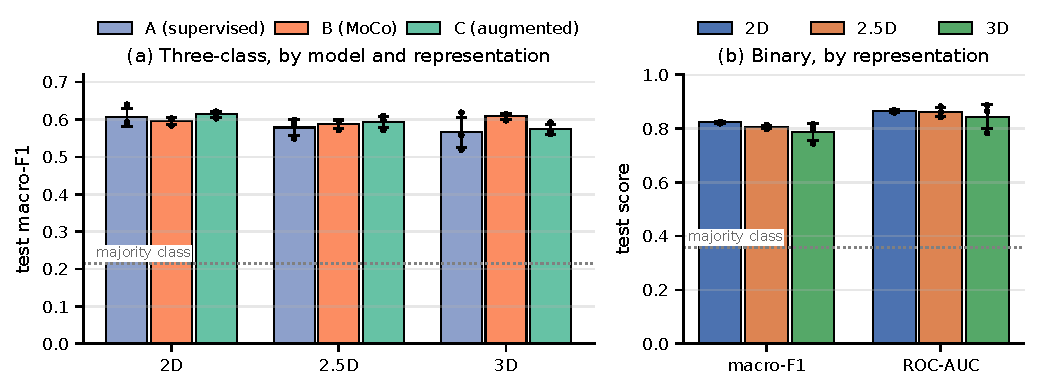
\includegraphics[width=\linewidth]{figures/fig_main_comparison.pdf}
\caption{Test performance by representation. Bars are means over three seeds,
error bars one standard deviation, dots individual seeds; the dotted line is the
majority-class baseline. (a)~Three-class macro-F1 for Models A--C. (b)~Binary
macro-F1 and ROC-AUC. No representation separates from the others.}
\label{fig:main}
\end{figure}

\begin{table}[t]\centering
\caption{Per-class test F1 (three-class), mean over three seeds. Malignant is
the easiest class and benign the hardest in every arm.}
\label{tab:perclass}
\begin{tabular}{llccc}
\toprule
Model & Class & 2D & 2.5D & 3D \\
\midrule
A (supervised) & benign        & $0.5362$ & $0.5328$ & $0.4583$ \\
               & indeterminate & $0.6001$ & $0.5550$ & $0.5733$ \\
               & malignant     & $0.6814$ & $0.6477$ & $0.6643$ \\
\midrule
B (MoCo)       & benign        & $0.5169$ & $0.4906$ & $0.4860$ \\
               & indeterminate & $0.6080$ & $0.5801$ & $0.6315$ \\
               & malignant     & $0.6623$ & $0.6917$ & $0.7074$ \\
\midrule
C (augmented)  & benign        & $0.5421$ & $0.5228$ & $0.4436$ \\
               & indeterminate & $0.6274$ & $0.5853$ & $0.5809$ \\
               & malignant     & $0.6708$ & $0.6720$ & $0.6970$ \\
\bottomrule
\end{tabular}
\end{table}

\begin{table}[t]\centering
\caption{Computational cost. Supervised minutes are per seed for Models A / B /
C; MoCo pretraining is a single run shared by the three Model B seeds. Times
were measured on different hardware and are not directly comparable across
arms.}
\label{tab:cost}
\begin{tabular}{lllccl}
\toprule
Arm & Encoder & Parameters & Supervised min/seed & MoCo min & Hardware \\
\midrule
2D   & ResNet-18    & 11{,}171{,}779 & 2.1 / 2.2 / 2.4    & 57.0  & Apple M2 \\
2.5D & ResNet-18    & 11{,}184{,}323 & 3.2 / 3.0 / 3.4    & 35.2  & Apple M2 \\
3D   & 3D ResNet-10 & 14{,}357{,}059 & 24.5 / 31.7 / 42.7 & 327.1 & Kaggle GPU \\
\bottomrule
\end{tabular}
\end{table}

\begin{figure}[t]\centering
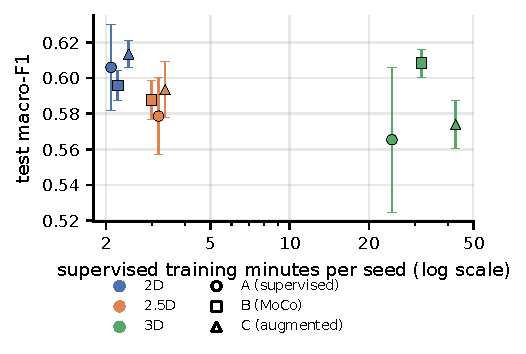
\includegraphics[width=0.55\linewidth]{figures/fig_cost.pdf}
\caption{Test macro-F1 against supervised training time per seed (log scale).
Error bars are one standard deviation over seeds. 3D costs more than an order
of magnitude more time without a corresponding gain.}
\label{fig:cost}
\end{figure}

Table~\ref{tab:main} and Figure~\ref{fig:main} show no benefit from additional
spatial context. Moving
from one slice to five changes three-class macro-F1 by $-0.027$ (Model A) and
$-0.020$ (Model C); extending to the full 104-slice volume changes it by
$-0.041$ and $-0.040$ respectively. With per-seed bootstrap intervals spanning
roughly $\pm0.05$ on a 396-nodule test set, none of these are distinguishable
from zero, and all are negative in sign. The strongest model overall is 2D
(Model C, $0.6134$); the strongest 3D model (Model B) reaches $0.6083$, an
indistinguishable figure that required a $327$-minute pretraining run plus
$31.7$ minutes of fine-tuning per seed on a Kaggle GPU, against $2.4$ minutes
per seed for 2D Model C on an Apple M2. Because the arms ran on different
hardware these times are not a controlled cost comparison, but they put 3D more
than an order of magnitude above 2D (Table~\ref{tab:cost},
Figure~\ref{fig:cost}). Binary ROC-AUC is nearly identical across
representations ($0.8644$, $0.8612$, $0.8443$), indicating that ranking
quality---not merely the decision threshold---is unchanged. Per-class F1
(Table~\ref{tab:perclass}) follows the same ordering in every arm: malignant is
easiest and benign hardest, despite benign being the larger training class.

\subsection{Self-supervised pretraining helps only the 3D encoder}

MoCo~v2 changed three-class test macro-F1 by $-0.0102$ in 2D and $+0.0090$ in
2.5D: opposite signs, both inside the seed spread. ROC-AUC was essentially
unchanged in 2D ($0.7579$ vs $0.7565$). The pretext task itself trained well,
with InfoNCE loss falling from $7.48$ to $4.14$ and instance-discrimination
accuracy reaching $0.863$ over 200 epochs (Figure~\ref{fig:moco}), so in these
two representations the outcome is a transfer failure rather than an
optimisation failure. Instance
discrimination rewards features that identify a crop---surrounding vasculature,
pleural contact, framing---which need not be the features that indicate
malignancy risk.

The 3D arm behaves differently. There MoCo gives $+0.043$ macro-F1 over the
supervised baseline ($0.6083$ vs $0.5653$) and $+0.035$ over the augmented model
($0.5738$), making the pretrained model the strongest 3D configuration we
obtained. The pattern across representations is consistent with pretraining
mattering in proportion to how data-starved supervised training is: the 3D
encoder carries $14.4$M parameters against $1876$ training volumes, where the
2D encoder sees the same patients as $11.2$M parameters over far simpler inputs.

We report this as an observation rather than a claim. In the 3D arm, validation
macro-F1 ranked the three configurations differently from test: validation
ordered them A ($0.5698$), B ($0.5662$), C ($0.5375$), whereas test ordered them
B, C, A. Model B scored below Model A on validation yet $0.043$ above it on
test, so with three seeds we cannot separate a genuine pretraining benefit from
checkpoint-selection noise. Distinguishing the two requires more seeds than we
ran.

\begin{figure}[t]\centering
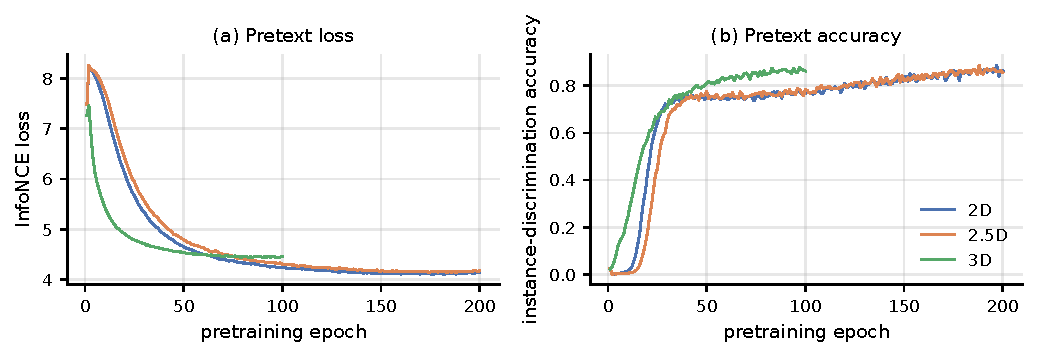
\includegraphics[width=\linewidth]{figures/fig_moco.pdf}
\caption{MoCo~v2 pretext training on the 5133-nodule pool. All three encoders
learn the pretext task; 3D uses a 100-epoch schedule.}
\label{fig:moco}
\end{figure}

\subsection{Augmentation does not reduce memorisation}

\begin{figure}[t]\centering
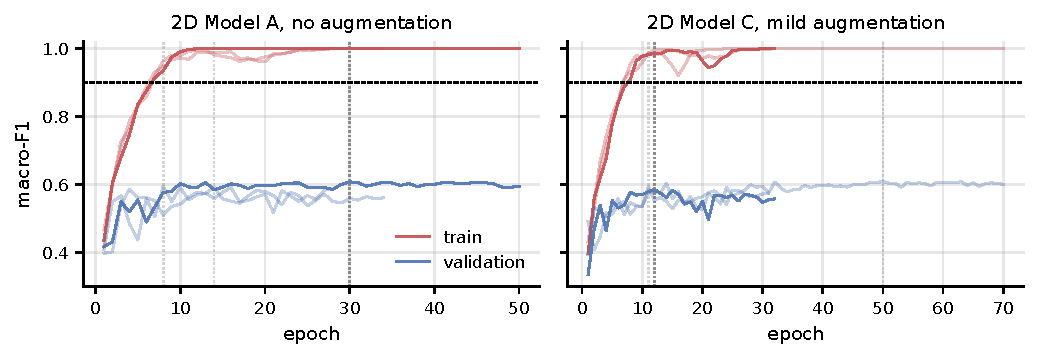
\includegraphics[width=\linewidth]{figures/fig_curves.pdf}
\caption{2D training and validation macro-F1 per epoch, without and with mild
augmentation. Seed 0 is drawn solid, seeds 1--2 faded; dotted verticals mark
the selected epochs and the dashed line marks $0.90$. Training macro-F1 passes
$0.90$ within 7--8 epochs either way while validation plateaus near $0.6$.}
\label{fig:curves}
\end{figure}

On test, mild augmentation gave the highest 2D score ($0.6134$ vs $0.6059$
unaugmented) and strong augmentation the lowest ($0.5908$). These differences
are inside the seed spread, and validation did not reproduce the ordering
($0.5982$, $0.5962$ and $0.5823$ for none, mild and strong), so we do not claim
an optimal strength. The train--validation macro-F1 gap at the selected epoch
(Figure~\ref{fig:curves})
was unchanged: $+0.386$ without augmentation, $+0.394$ with mild augmentation.
Peak 2D training macro-F1 reached $1.000$ with and without mild augmentation
($0.999$ with strong augmentation), and training
macro-F1 crossed $0.90$ at epoch 7--8 regardless of augmentation. What
augmentation reliably delivered was \emph{stability}: the seed standard
deviation of test macro-F1 fell from $\pm0.024$ to $\pm0.008$. Early stopping,
not augmentation, is what limits overfitting here.

\subsection{The ceiling is annotator disagreement}
\label{sec:ceiling}

\begin{table}[t]\centering
\caption{Binary test performance stratified by label confidence
(2D, probabilities averaged over three seeds). ``Confident'' means no midpoint
median, at least three readers, and no disagreement flag.}
\label{tab:ceiling}
\begin{tabular}{lccc}
\toprule
Subset & $n$ & Accuracy & AUC \\
\midrule
Confident labels & 55 & $0.945$ & $0.987$ \\
Remainder        & 154 & $0.805$ & $0.902$ \\
\bottomrule
\end{tabular}
\end{table}

\begin{figure}[t]\centering
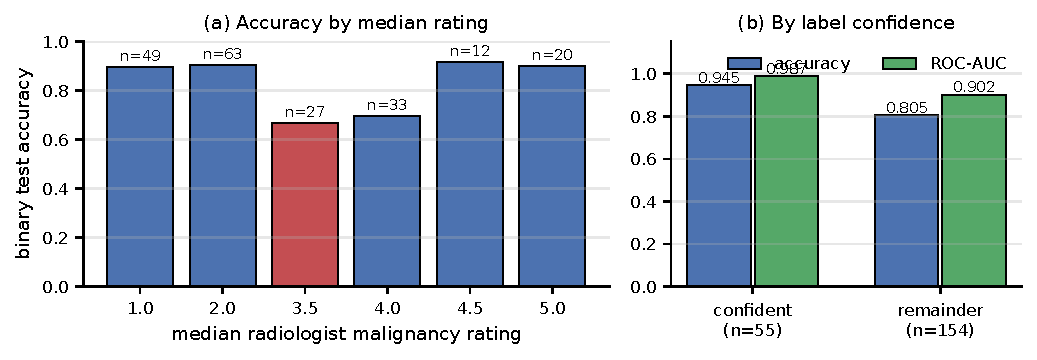
\includegraphics[width=\linewidth]{figures/fig_ceiling.pdf}
\caption{Binary test accuracy against label confidence (2D, probabilities
averaged over three seeds). (a)~By median radiologist rating; the red bar is a
midpoint median ($3.5$), which no radiologist assigned. (b)~By the confidence
subsets of Table~\ref{tab:ceiling}.}
\label{fig:ceiling}
\end{figure}

\begin{figure}[t]\centering
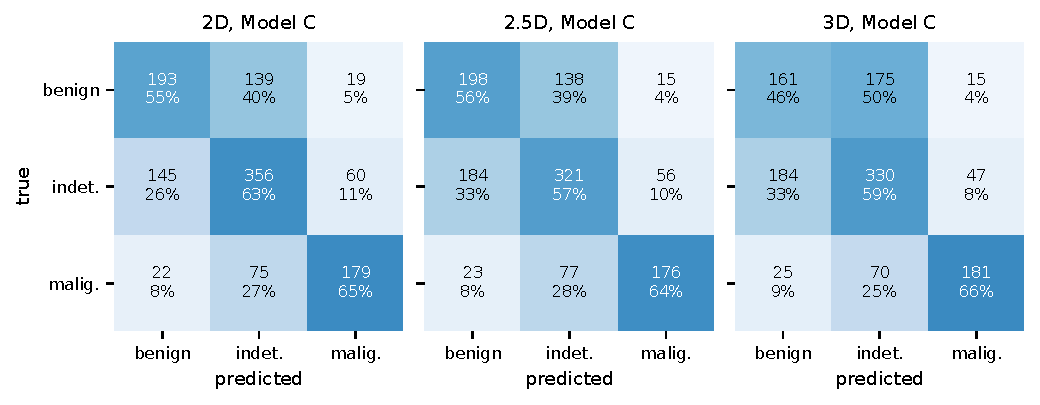
\includegraphics[width=\linewidth]{figures/fig_confusion.pdf}
\caption{Three-class test confusion matrices for Model C, pooled over three
seeds (counts and row percentages). Errors concentrate on the
benign/indeterminate and indeterminate/malignant boundaries in every arm.}
\label{fig:confusion}
\end{figure}

Table~\ref{tab:ceiling} and Figure~\ref{fig:ceiling} are our central result. On nodules where radiologists
agreed, a single-slice ResNet-18 reaches $0.945$ accuracy and $0.987$ AUC. The
pooled accuracy of the same seed-averaged predictions, $0.842$ ($176/209$), is
depressed almost entirely by nodules where they did not.

Accuracy tracks the median rating directly: $0.898$ at median $1.0$, $0.905$ at
$2.0$, $0.900$ at $5.0$---but $0.667$ at $3.5$ and $0.697$ at $4.0$. Recall that
$3.5$ is not a rating any radiologist assigned. Nodules flagged as midpoint
medians score $0.667$ against $0.868$ for the rest; single-reader nodules score
$0.722$ against $0.903$ for three-reader nodules.

The three-class confusion matrices (Figure~\ref{fig:confusion}) show the same
structure. Pooling over seeds for 2D Model C,
benign$\leftrightarrow$indeterminate accounts for 284 errors and
indeterminate$\leftrightarrow$malignant for 135, while
benign$\leftrightarrow$malignant accounts for only 41. The 2.5D (322 / 133 / 38)
and 3D (359 / 117 / 40) arms follow the same pattern. The clinically meaningful
extremes are separable; the boundary that is not is the one defined by reader
disagreement.

Finally, the models are markedly less confident when they are wrong: mean
confidence is $0.762$ on correct predictions and $0.462$ on errors, and 19 of
33 binary errors fall at median $3.5$ or $4.0$.

\section{Discussion}

Three architectures spanning one to 104 slices, each additionally pretrained on
5133 unlabelled volumes, converge to the same three-class performance: the best
configuration of every representation lands between $0.5934$ and $0.6134$
macro-F1. The most parsimonious explanation is that they are all saturating the
information available in the labels rather than in the images. On that reading,
pretraining helps the 3D encoder not by supplying information the images lacked
but by partially compensating for the optimisation disadvantage of fitting
$14.4$M parameters to $1876$ volumes---it moves the weakest representation up
to the common ceiling rather than through it.

This has a practical consequence for the literature. Improvements of one or two
macro-F1 points on LIDC-IDRI, reported without stratification by annotator
agreement and without confidence intervals, are difficult to distinguish from
noise: on a 396-nodule test set our bootstrap intervals span $\pm0.05$. We
recommend that LIDC-IDRI results be reported separately for unanimously and
ambiguously labelled nodules, and that midpoint medians---which are averaging
artefacts, not clinical categories---be flagged explicitly.

\section{Limitations}

The labelled cohort is small (1876 training nodules) relative to encoder
capacity, and all models overfit substantially. Confidence intervals are
correspondingly wide, and we have deliberately refrained from claiming that any
representation is superior. Labels are radiologist opinion rather than
histopathology, so the ``ceiling'' we measure is agreement with readers, not
with ground truth. We evaluated a single self-supervised configuration per
representation, and the 3D one used a shorter schedule than 2D and 2.5D; a
negative transfer result for one MoCo~v2 setting is not evidence that
self-supervision cannot help. In the reported 3D runs that use augmentation
(Model C, binary, and the MoCo views behind Model B), rotation was applied in
the sagittal rather than the axial plane, so 3D augmentation is not an exact
analogue of the 2D recipe; Model A is unaffected. Training times were measured
on different hardware across arms. Each configuration was run with three seeds;
this is enough to show that the representations do not separate, but not enough
to resolve the $+0.043$ pretraining effect in the 3D arm, particularly as 3D
validation macro-F1 ranked configurations inconsistently with test. The $z$ axis
was resampled from $2.5\,\mathrm{mm}$, so inter-slice context is partly
interpolated, which disadvantages the 2.5D and 3D arms to an unknown degree.
Hyperparameters were tuned on a 382-nodule validation split, itself a small
sample, and the search was conducted on the 2D arm and transferred unchanged to
2.5D and 3D. Holding hyperparameters fixed isolates the effect of the
representation, but it does not give each architecture its best achievable
configuration, and a per-arm search could narrow or widen the gaps we report.

\section{Conclusion}

Under a controlled single-pipeline comparison, additional spatial context did
not improve pulmonary nodule malignancy-risk classification on LIDC-IDRI, and
self-supervised pretraining improved only the representation that was furthest
behind, without lifting it past the others. Performance is instead bounded by
annotator disagreement: where radiologists agree, a single CT slice suffices for
$0.945$ accuracy and $0.987$ AUC. We suggest that progress on this benchmark be
measured against agreement-stratified baselines.

\paragraph{Code and reproducibility.} All code, per-seed metrics, training
curves and confusion matrices are available at
\url{https://github.com/naazzarov/CT-2D-2.5D-3D-DeepLearning}.

\bibliographystyle{plainnat}
\bibliography{refs}

\end{document}
